\documentclass[10pt]{article}

\usepackage[T1]{fontenc}
\usepackage{geometry}
\usepackage{amsmath, amssymb, amsthm}
\usepackage{graphicx}
\usepackage{subcaption}
\usepackage{float}
\usepackage{multirow}
\usepackage{bm}
\usepackage{hyperref}

\geometry{a4paper, margin=1in}


\newcommand{\C}{\mathbb{C}}
\newcommand{\R}{\mathbb{R}}
\newcommand{\Q}{\mathbb{Q}}
\newcommand{\Z}{\mathbb{Z}}
\newcommand{\N}{\mathbb{N}}
\newcommand{\E}{\mathbb{E}}
\newcommand{\iid}{\overset{\text{iid}}{\sim}}
\newcommand{\topr}{\overset{p\,}{\longrightarrow}}

\setlength{\parindent}{0em}

\title{Assignment}
\author{Satvik Saha}
\date{}

\begin{document}
    \noindent\textbf{IISER Kolkata} \hfill \textbf{Assignment}
    \vspace{3pt}
    \hrule
    \vspace{3pt}
    \begin{center}
    \LARGE{\textbf{MA5208: Introduction to Bayesian Analysis}}
    \end{center}
    \vspace{3pt}
    \hrule
    \vspace{3pt}
    Satvik Saha, \texttt{19MS154} \hfill \today
    \vspace{20pt}

    \setlength{\parskip}{1em}


    \section*{Problem 1}

    We estimate \[
        I = \int_2^\infty \frac{1}{\pi(1 + x^2)} \:dx
    \] via Monte-Carlo methods.
    First, note that this is simply $\E[\bm{1}_{[2, \infty)}(X)]$ where $X
    \sim \text{Cauchy}(0, 1)$.
    Thus, we sample $X_1, \dots, X_n \iid \text{Cauchy}(0, 1)$, and estimate
    \[
        \hat{I}_{\text{Cauchy}} \;=\; \frac{1}{n} \sum_{i = 1}^n \bm{1}_{[2, \infty)}(X_i) \;\topr\; I.
    \]

    Next, note that for $U \sim \text{Uniform}(2, M)$ and $M \gg 2$, we have
    \[
        I \;=\; \E\left[\frac{1}{\pi(1 + U^2)}\cdot \frac{1}{f_U(u)}\right] + \int_M^\infty \frac{1}{\pi(1 + x^2)} \:dx,
    \] where the last term is very small; indeed, \[
        \int_M^\infty \frac{1}{\pi(1 + x^2)} \:dx < \int_M^\infty \frac{1}{\pi x^2} \:dx = \frac{1}{\pi M}.
    \]
    We fix $M = 1000$, sample $U_1, \dots, U_n \iid \text{Uniform}(2, M)$, and
    estimate \[
        \hat{I}_{\text{Uniform,I}} \;=\; \frac{1}{n} \sum_{i = 1}^n \frac{1}{\pi(1 + U_i^2)} \cdot (M - 2) \;\topr\; \int_2^M \frac{1}{\pi(1 + x^2)} \:dx \approx I.
    \]

    In fact, we could also use the idea \[
        I = \frac{1}{2} - \int_0^2 \frac{1}{\pi(1 + x^2)}
    \] and sample $V_1, \dots, V_n \iid \text{Uniform}(0, 2)$, then estimate
    \[
        \hat{I}_{\text{Uniform,II}} \;=\; \frac{1}{2} - \frac{1}{n} \sum_{i = 1}^n \frac{1}{\pi(1 + V_i^2)} \cdot 2 \;\topr\; I.
    \]

    These methods have been illustrated in Figure~\ref{fig:P1}. For $n = 10^7$
    sample points, we obtain the estimates
    \begin{align*}
        \hat{I}_{\text{Cauchy}} \;&=\; 0.1475, \\
        \hat{I}_{\text{Uniform,I}} \;&=\; 0.1479, \\
        \hat{I}_{\text{Uniform,II}} \;&=\; 0.1476.
    \end{align*}
    The true value is $1/2 - \arctan(2)/\pi \approx 0.1476$.

    \begin{figure}[H]
        \centering
        \begin{subfigure}{\textwidth}
            \centering
            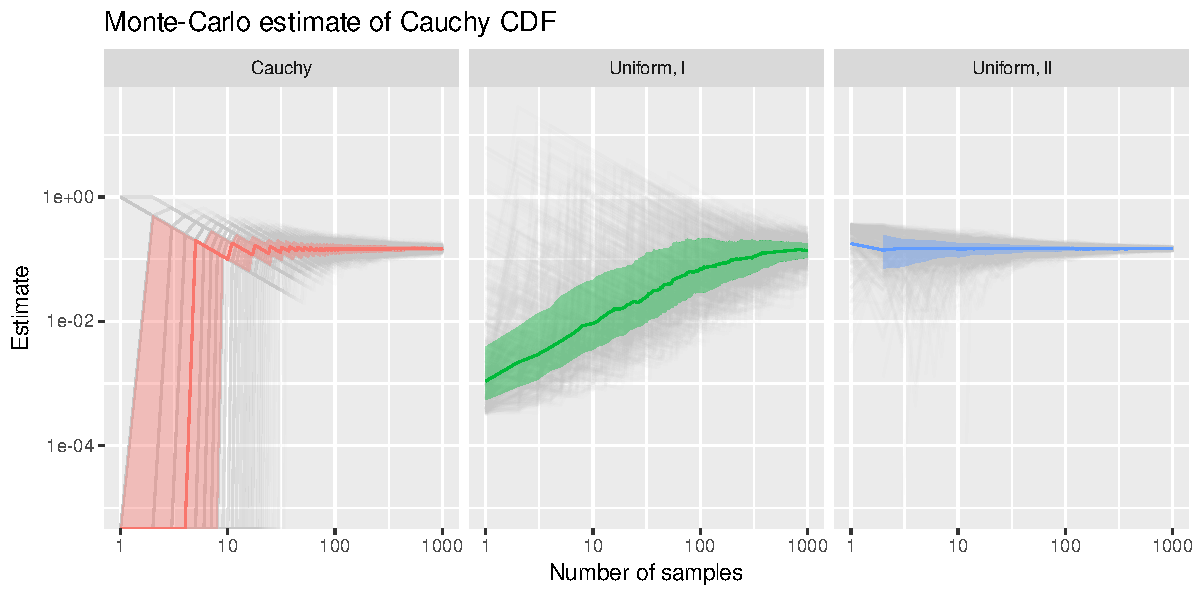
\includegraphics[width=\textwidth, page=1]{cauchy}
            \caption{
                Trace plots of estimates of $I$, obtained via Monte-Carlo
                sampling from Student's $t_{12}$, Cauchy, and Gamma
                distributions, using $n$ sample points.
                The colored line indicates the median of the estimates, and
                the ribbon encloses the first and third quartiles.
            }
            \label{fig:P1_trace}
        \end{subfigure}

        \vspace{2em}
        \begin{subfigure}{\textwidth}
            \centering
            \includegraphics[width=\textwidth, page=2]{cauchy}
            \caption{
                Inter-quartile ranges of estimates of $I$ against number of
                samples drawn.
            }
            \label{fig:P1_IQR}
        \end{subfigure}
        \caption{Estimation of $I$ via Monte-Carlo methods.}
        \label{fig:P1}
    \end{figure}


    \clearpage

    \section*{Problem 2}

    We estimate \[
        I = \E_{X \sim t_{12}}[h(X)], \qquad h(x) = \sqrt{\frac{|x|}{|1 - x|}}.
    \]
    First, we sample $X_1, \dots, X_n \iid t_{12}$, and estimate \[
        \hat{I}_{t_{12}} = \frac{1}{n} \sum_{i = 1}^n h(X_i) \topr I.
    \] Next, we sample $Y_1, \dots, Y_n \iid \text{Cauchy}(0, 1)$, and
    estimate \[
        \hat{I}_{\text{Cauchy}} = \frac{1}{n}\sum_{i = 1}^n h(Y_i)\cdot \frac{f_X(Y_i)}{f_Y(Y_i)} \topr I,
    \] where $f_X$ is the density function of $X_1 \sim t_{12}$, and $f_Y$ is
    the density function of $Y_1 \sim \text{Cauchy}(0, 1)$.
    Finally, we sample $\tilde{Z}_1, \dots, \tilde{Z}_n \iid \text{Gamma}(1/2,
    1)$, and iid $U_1, \dots, U_n$ where each $P(U_i = 1) = P(U_i = -1) =
    1/2$. Then, we set $Z_i = U_i\tilde{Z}_i + 1$; observe that $|Z_i - 1|
    \iid \text{Gamma}(1/2, 1)$. Also, if $f_{\tilde{Z}}$ denotes the density
    function of $\tilde{Z}_1 \sim \text{Gamma}(1/2, 1)$, then \[
        f_Z(z) = \frac{1}{2}f_{\tilde{Z}}(|z - 1|).
    \] Using this, we estimate \[
        \hat{I}_{\text{Gamma}} = \frac{1}{n}\sum_{i = 1}^n h(Z_i)\cdot \frac{f_X(Z_i)}{f_Z(Z_i)} \topr I.
    \]

    These methods have been illustrated in Figure~\ref{fig:P2}. For $n = 10^7$
    sample points, we obtain the estimates
    \begin{align*}
        \hat{I}_{t_{12}} \;&=\; 1.1603, \\
        \hat{I}_{\text{Cauchy}} \;&=\; 1.1600, \\
        \hat{I}_{\text{Gamma}} \;&=\; 1.1605.
    \end{align*}


    \begin{figure}[H]
        \centering
        \begin{subfigure}{\textwidth}
            \centering
            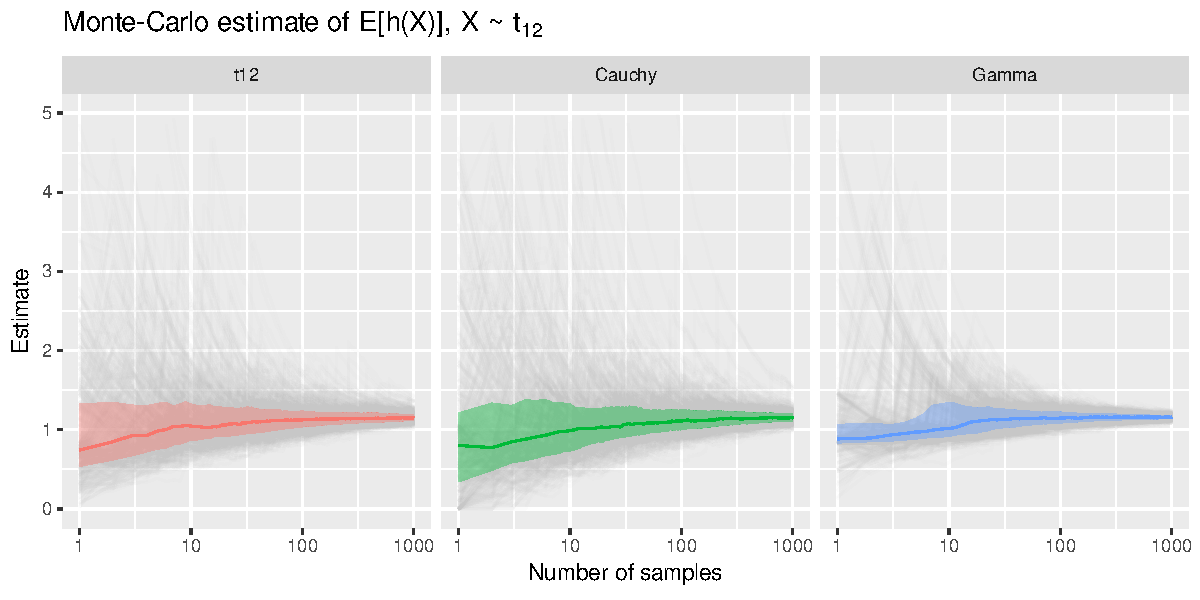
\includegraphics[width=\textwidth, page=1]{t12}
            \caption{
                Trace plots of estimates of $I$, obtained via Monte-Carlo
                sampling from a Cauchy and uniform distributions, using $n$
                sample points.
                The colored line indicates the median of the estimates, and
                the ribbon encloses the first and third quartiles.
            }
            \label{fig:P2_trace}
        \end{subfigure}

        \vspace{2em}
        \begin{subfigure}{\textwidth}
            \centering
            \includegraphics[width=\textwidth, page=2]{t12}
            \caption{
                Inter-quartile ranges of estimates of $I$ against number of
                samples drawn.
            }
            \label{fig:P2_IQR}
        \end{subfigure}
        \caption{Estimation of $I$ via Monte-Carlo methods.}
        \label{fig:P2}
    \end{figure}


    \clearpage

    \section*{Problem 3}

    We fix our covariates $\bm{X} = [x_{it}]_{1 \leq i \leq I, 1 \leq t \leq
    T}$, and have our responses $\bm{Y} = [y_{it}]$.
    Let $g(\cdot)$ denote the full conditional of the parameter $(\cdot)$.
    Then, we have the following.
    \begin{align*}
        g(y_{it}) &\propto f(y_{it} \mid \theta_{it} = \alpha_t + \beta_t x_{it} + \epsilon_{it}), \\
        g(\epsilon_{it}) &\propto f(\epsilon_{it}\mid \sigma^2_t)\, f(y_{it}\mid \theta_{it}), \\
        g(\sigma^2_t) &\propto f(\sigma^2_t)\, \prod_{i = 1}^I f(\epsilon_{it}\mid \sigma^2_t), \\
        g(\alpha_0) &\propto f(\alpha_0)\, f(\alpha_1\mid \alpha_0, \tau^2_\alpha), \\
        g(\alpha_t) &\propto f(\alpha_t\mid \alpha_{t - 1}, \tau^2_\alpha)\, f(\alpha_{t + 1}\mid \alpha_t, \tau^2_\alpha)\,\prod_{i = 1}^I f(y_{it}\mid \theta_{it}), \\
        g(\beta_0) &\propto f(\beta_0\mid \tau^2_\beta)\, f(\beta_1\mid \beta_0, \tau^2_\beta), \\
        g(\beta_t) &\propto f(\beta_t\mid \beta_{t - 1}, \tau^2_\beta)\, f(\beta_{t + 1}\mid \beta_t, \tau^2_\beta)\, \prod_{i = 1}^I f(y_{it}\mid \theta_{it}), \\
        g(\tau^2_\alpha) &\propto f(\tau^2_\alpha)\, \prod_{t = 1}^T f(\alpha_t\mid \alpha_{t - 1}, \tau^2_\alpha), \\
        g(\tau^2_\beta) &\propto f(\tau^2_\beta)\, f(\beta_0\mid \tau^2_\beta)\, \prod_{t = 1}^T f(\beta_t\mid \beta_{t - 1}, \tau^2_\beta).
    \end{align*}
    Now, \begin{align*}
        f(y_{it}\mid \theta_{it}) &\propto \frac{e^{\theta_{it} y_{it}}}{\Gamma(y_{it} + 1)} e^{-e^{\theta_{it}}} \sim\mathcal{P}(e^{\theta_{it}}), \\
        f(\epsilon_{it}\mid \sigma^2_t) &\propto (\sigma^2_t)^{-1/2} e^{-\epsilon_{it}^2 / 2\sigma^2_t} \sim \mathcal{N}(0, \sigma^2_t), \\
        f(\sigma^2_t) &\propto (\sigma^2_t)^{-2} e^{-1/\sigma^2_t} \sim \mathcal{IG}(1, 1), \\
        f(\alpha_0) &\propto e^{-\alpha_0^2 / 200} \sim \mathcal{N}(0, 100), \\
        f(\alpha_t\mid \alpha_{t - 1}, \tau^2_\alpha) &\propto (\tau^2_\alpha)^{-1/2} e^{-(\alpha_t - \alpha_{t - 1})^2 / 2\tau^2_\alpha} \sim \mathcal{N}(\alpha_{t - 1}, \tau^2_\alpha), \\
        f(\beta_0\mid \tau^2_\beta) &\propto (\tau^2_\beta)^{-1/2} e^{-\beta_0^2 / 2\tau^2_\beta} \sim \mathcal{N}(0, \tau^2_\beta), \\
        f(\beta_t\mid \beta_{t - 1}, \tau^2_\beta) &\propto (\tau^2_\beta)^{-1/2} e^{-(\beta_t - \beta_{t - 1})^2 / 2\tau^2_\beta} \sim \mathcal{N}(\beta_{t - 1}, \tau^2_\beta), \\
        f(\tau^2_\alpha) &\propto (\tau^2_\alpha)^{-2} e^{-1/\tau^2_\alpha} \sim \mathcal{IG}(1, 1), \\
        f(\tau^2_\beta) &\propto (\tau^2_\beta)^{-2} e^{-1/\tau^2_\beta} \sim \mathcal{IG}(1, 1).
    \end{align*}

    Thus,
    \begin{align*}
        g(y_{it}) &\sim \mathcal{P}(e^{\theta_{it} y_{it}}), \\
        g(\sigma^2_t) &\propto (\sigma^2_t)^{-(2 + I/2)} e^{-\left(2 + \sum_{i = 1}^I \epsilon_{it}^2\right) / 2\sigma^2_t} \sim \mathcal{IG}\left(1 + I/2,\, 1 + \frac{1}{2}\sum_{i = 1}^I \epsilon_{it}^2\right), \\
        g(\alpha_0) &\propto e^{-\alpha_0^2/200 - (\alpha_1 - \alpha_0)^2 / 2\tau^2_\alpha} \sim \mathcal{N}\left(\frac{100 \alpha_1}{100 + \tau^2_\alpha},\, \frac{100\tau^2_\alpha}{100 + \tau^2_\alpha}\right), \\
        g(\beta_0) &\propto e^{-\beta_0^2/2\tau^2_\beta - (\beta_1 - \beta_0)^2/2\tau^2_\beta} \sim \mathcal{N}(\beta_1 / 2,\, \tau^2_\beta/2), \\
        g(\tau^2_\alpha) &\propto (\tau^2_\alpha)^{-2} e^{-1/\tau^2_\alpha} (\tau^2_\alpha)^{-T/2} e^{-\sum_{t = 1}^T (\alpha_t - \alpha_{t - 1}^2) / 2\tau^2_\alpha} \sim \mathcal{IG}\left(1 + T/2,\, 1 + \frac{1}{2}\sum_{t = 1}^T (\alpha_t - \alpha_{t - 1})^2\right), \\
        g(\tau^2_\beta) &\propto (\tau^2_\beta)^{-2 - (T + 1)/2} e^{-1/\tau^2_\beta - \beta_0^2 / 2\tau^2_\beta - \sum_{t = 1}^T (\beta_t - \beta_{t - 1})^2 / 2\tau^2\beta} \sim \mathcal{IG}\left(1 + (T + 1)/2,\, 1 + \frac{\beta_0^2}{2} + \frac{1}{2}\sum_{t = 1}^T (\beta_t - \beta_{t - 1})^2\right).
    \end{align*}

    The remaining full conditionals do not resolve into standard
    distributions; they will be sampled via the Metropolis-Hastings algorithm.

    For instance, to sample from $g(\alpha_t)$, we may use a proposal
    distribution of the form $q(\cdot\mid x) = \mathcal{N}(x, \tau^2_\alpha)$.



\end{document}
